% !TEX program = xelatex
\documentclass[a4paper,10pt]{article}

\makeatletter
\let\@expl@@@mark@update@singlecol@structures@@\relax
\makeatother

\usepackage[a4paper, left=1.0cm, right=1.0cm, top=0.90cm, bottom=1.05cm, footskip=0.48cm]{geometry}
\usepackage{fontspec}
\usepackage{amsmath, amssymb}
\usepackage{array, colortbl}
\usepackage[table]{xcolor}
\usepackage{tcolorbox}
\tcbuselibrary{skins, breakable}
\usepackage{fancyhdr}
\usepackage{enumitem}
\usepackage{tikz}
\usetikzlibrary{calc, angles, quotes, arrows.meta}

\makeatletter
\newcommand{\NGSFindFonts}{%
  \IfFileExists{../../../fonts/KhmerOSsiemreap.ttf}{%
    \def\NGSUserPath{../../../fonts/}\def\NGSSysPath{../../../fonts/}%
  }{%
    \IfFileExists{../../../../fonts/KhmerOSsiemreap.ttf}{%
      \def\NGSUserPath{../../../../fonts/}\def\NGSSysPath{../../../../fonts/}%
    }{%
      \IfFileExists{fonts/KhmerOSsiemreap.ttf}{%
        \def\NGSUserPath{fonts/}\def\NGSSysPath{fonts/}%
      }{%
        \def\NGSUserPath{C:/Users/user/AppData/Local/Microsoft/Windows/Fonts/}%
        \def\NGSSysPath{C:/Windows/Fonts/}%
      }%
    }%
  }%
}
\NGSFindFonts
\makeatother

\XeTeXlinebreaklocale "km"
\XeTeXlinebreakskip = 0pt plus 1pt minus 0.1pt

\setmainfont[
  Path = {\NGSUserPath},
  Extension = .ttf,
  UprightFont = KhmerOSsiemreap,
  BoldFont = KhmerOSsiemreap,
  BoldFeatures = {FakeBold=1.8},
  ItalicFont = KhmerOSsiemreap,
  ItalicFeatures = {FakeSlant=0.25}
]{KhmerOSsiemreap}

\newfontfamily\muol[Path={\NGSUserPath}]{KhmerOSmuollight.ttf}
\newfontfamily\enfont[Path={\NGSSysPath}, Scale=1.0]{times.ttf}
\newfontfamily\enbold[Path={\NGSSysPath}, Scale=1.0]{timesbd.ttf}
\newfontfamily\calibrifont[Path={\NGSSysPath}, Scale=0.95]{calibri.ttf}

\DeclareTextFontCommand{\en}{\enfont}
\newcommand{\enbf}[1]{{\enbold #1}}

\definecolor{headgray}{HTML}{E2E2E2}
\definecolor{panelgray}{HTML}{F5F5F5}

\pagestyle{fancy}
\fancyhf{}
\renewcommand{\headrulewidth}{0pt}
\renewcommand{\footrulewidth}{0.4pt}
\fancyfoot[L]{\rule{0pt}{11pt}\fontsize{8.5pt}{11pt}\selectfont អនុវិទ្យាល័យព្រះក្រសាំង $\;\vert\;$ គណិតវិទ្យា ថ្នាក់ទី៨ $\;\vert\;$ មេរៀនទី១៥ (១៥.២.២) ធ្នូ និងអង្កត់ធ្នូ}
\fancyfoot[R]{\rule{0pt}{11pt}\fontsize{8.5pt}{11pt}\selectfont ទំព័រ \en{\thepage\,/\,2}}

\setlength{\parindent}{0pt}
\setlength{\tabcolsep}{4pt}

\newcommand{\tri}[1]{\triangle #1}
\newcommand{\unit}[1]{\,\text{\en{#1}}}
\newcommand{\blank}[1]{\leavevmode\hbox to #1{\dotfill}}
\newcommand{\chkbox}{\tikz[baseline=0.2ex]\draw[black, line width=0.7pt] (0,0) rectangle (1.55ex,1.55ex);}
\newcommand{\cnum}[1]{\tikz[baseline=-0.58ex]\node[circle, fill=black, text=white, inner sep=0.85pt, minimum size=1.95ex, font=\enbold\scriptsize]{#1};}

\newcommand{\arc}[1]{\mbox{%
  \tikz[baseline=(arcX.base)]{%
    \node[inner sep=0pt, outer sep=0pt] (arcX) {$#1$};%
    \draw[black, line width=0.55pt] ($(arcX.north west)+(0.02,0.035)$) to[bend left=30] ($(arcX.north east)+(-0.02,0.035)$);%
  }%
}}

\newcommand{\tickone}[2]{%
  \coordinate (tkM) at ($(#1)!0.5!(#2)$);
  \draw[black, line width=0.7pt] ($(tkM)!0.11cm!90:(#2)$) -- ($(tkM)!0.11cm!-90:(#2)$);
}
\newcommand{\ticktwo}[2]{%
  \coordinate (tkM1) at ($(#1)!0.47!(#2)$);
  \coordinate (tkM2) at ($(#1)!0.53!(#2)$);
  \draw[black, line width=0.7pt] ($(tkM1)!0.11cm!90:(#2)$) -- ($(tkM1)!0.11cm!-90:(#2)$);
  \draw[black, line width=0.7pt] ($(tkM2)!0.11cm!90:(#2)$) -- ($(tkM2)!0.11cm!-90:(#2)$);
}

\newcommand{\secbar}[2]{%
  \vspace{2.5pt}%
  \begin{tcolorbox}[
    enhanced, sharp corners, colback=headgray, colframe=black,
    boxrule=0.85pt, left=6pt, right=6pt, top=2.5pt, bottom=2.5pt, after skip=3.5pt
  ]
    {\muol\fontsize{9.5pt}{14pt}\selectfont #1}\hfill{\fontsize{9pt}{13pt}\selectfont\textbf{#2}}
  \end{tcolorbox}%
}

\begin{document}
\fontsize{9.6pt}{14.2pt}\selectfont

% ==================== ក្បាលសន្លឹកកិច្ចការ ====================
\begin{tcolorbox}[
  enhanced, sharp corners, colback=white, colframe=black,
  boxrule=1.1pt, left=6pt, right=6pt, top=3.5pt, bottom=3.5pt, after skip=3pt
]
  \begin{minipage}[c]{11.2cm}
    {\muol\fontsize{10.5pt}{15.5pt}\selectfont សន្លឹកកិច្ចការសិស្ស — មេរៀនទី១៥ ៖ រង្វង់}\\[1.5pt]
    \textbf{ចំណុច ២.១ ៖ ធ្នូ និងអង្កត់ធ្នូ} (សៀវភៅគោល ទំ.២០០--២០១ និង ២០៤)
  \end{minipage}\hfill
  \begin{minipage}[c]{6.7cm}
    ឈ្មោះសិស្ស៖ \blank{4.4cm}\\[2pt]
    ថ្នាក់ទី៨៖ \blank{1.3cm} \hspace{0.2cm} ដៃគូទី៖ \blank{2.0cm}
  \end{minipage}
\end{tcolorbox}

% ==================== ផ្នែកទី ១ ៖ E1 - ENGAGE ====================
\secbar{ផ្នែកទី ១ ៖ បេសកកម្មជាងត្បាញចង្អេរឫស្សី (\enbf{E1}) — របារឫស្សីត្រង់វែងបំផុត}{\en{3} នាទី (ទស្សន៍ទាយមុនរៀន)}

\begin{tcolorbox}[
  enhanced, sharp corners, colback=panelgray, colframe=black,
  boxrule=0.8pt, left=6pt, right=6pt, top=3pt, bottom=3pt, after skip=3pt
]
  \begin{minipage}[c]{12.4cm}
    ជាងត្បាញចង្អេរឫស្សីមូលមួយដែលមានកាំ $r = 25\unit{cm}$ ចង់ដាក់ \textbf{របារឫស្សីត្រង់ ១ ដើម} ភ្ជាប់គែមចង្អេរពីម្ខាងទៅម្ខាងឱ្យមានប្រវែងវែងជាងគេបំផុតដើម្បីទប់កុំឱ្យវៀច។ ចូរទស្សន៍ទាយ៖\\[2pt]
    ១. តើត្រូវដាក់របារកាត់តាមណា? \hspace{0.12cm} \mbox{\chkbox\ ក្បែរគែម} \hspace{0.18cm} \mbox{\chkbox\ កាត់តាមផ្ចិត $O$} \hspace{0.18cm} \mbox{\chkbox\ កន្លែងណាក៏ស្មើគ្នា}\\[2pt]
    ២. បើធ្នូ $\arc{CF}$ ធំជាងធ្នូ $\arc{CD}$ ពីរដង ($\arc{CF} = 2\arc{CD}$) តើអង្កត់ធ្នូ $CF$ និង $2CD$ យ៉ាងដូចម្ដេច? \hspace{0.1cm} \mbox{\chkbox\ $CF = 2CD$} \hspace{0.15cm} \mbox{\chkbox\ $CF < 2CD$}
  \end{minipage}\hfill
  \begin{minipage}[c]{5.6cm}
    \centering
    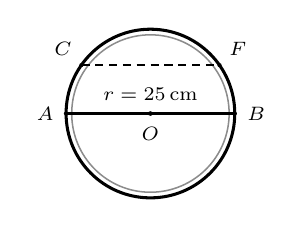
\begin{tikzpicture}[scale=0.42, every node/.style={font=\scriptsize, text=black}]
      \coordinate (O) at (0,0);
      \def\R{2.55}
      \draw[black, line width=1.1pt] (O) circle (\R);
      \draw[black!45, line width=0.55pt] (O) circle (2.38);
      \draw[black, line width=1.1pt] (-\R,0)--(\R,0);
      \draw[black, line width=0.85pt, densely dashed] (145:\R)--(35:\R);
      \fill[black] (O) circle (2pt) (-\R,0) circle (1.9pt) (\R,0) circle (1.9pt) (145:\R) circle (1.8pt) (35:\R) circle (1.8pt);
      \node[below=1.5pt] at (O) {$O$};
      \node[left=1pt] at (-\R,0) {$A$}; \node[right=1pt] at (\R,0) {$B$};
      \node[above left=0pt] at (145:\R) {$C$}; \node[above right=0pt] at (35:\R) {$F$};
      \node[above=1pt] at (0,0) {$r=25\unit{cm}$};
    \end{tikzpicture}
  \end{minipage}
\end{tcolorbox}

% ==================== ផ្នែកទី ២ ៖ E2 - EXPLORE ====================
\secbar{ផ្នែកទី ២ ៖ ពិសោធន៍វាស់ប្រវែងពិត (មាត្រដ្ឋាន \enbf{1:1}) និងអន្ទាក់មិនសមាមាត្រ (\enbf{E2 — Explore})}{\en{11} នាទី (ពិភាក្សាដៃគូ)}

\begin{minipage}[c]{5.5cm}
  \centering
  \begin{tikzpicture}[x=1cm, y=1cm, every node/.style={font=\footnotesize, text=black}]
    % រង្វង់មាត្រដ្ឋានពិត 1:1 កាំ r = 2.0 cm (អង្កត់ផ្ចិត AB = 4.0 cm)
    \coordinate (O) at (0,0);
    \def\R{2.0}
    \coordinate (A) at (-\R,0);
    \coordinate (B) at (\R,0);
    \coordinate (C) at (150:\R);
    \coordinate (D) at (90:\R);
    \coordinate (F) at (30:\R);
    \coordinate (E) at (-90:\R);
    \coordinate (G) at (-30:\R);
    \draw[black, line width=1.05pt] (O) circle (\R);
    \draw[black, line width=1.1pt] (A)--(B);
    \draw[black, line width=0.95pt] (C)--(D) (E)--(G) (C)--(F);
    \draw[black!60, line width=0.7pt, densely dashed] (O)--(C) (O)--(D) (O)--(F) (D)--(F);
    \fill[black] (O) circle (2.1pt) (A) circle (2pt) (B) circle (2pt) (C) circle (2pt) (D) circle (2pt) (F) circle (2pt) (E) circle (2pt) (G) circle (2pt);
    \node[below left=0.5pt] at (O) {$O$};
    \node[left=1pt] at (A) {$A$};
    \node[right=1pt] at (B) {$B$};
    \node[above left=0.5pt] at (C) {$C$};
    \node[above=1pt] at (D) {$D$};
    \node[above right=0.5pt] at (F) {$F$};
    \node[below=1pt] at (E) {$E$};
    \node[below right=0.5pt] at (G) {$G$};
    \node[align=center, font=\scriptsize] at (0,-2.78) {$C(O, 2\unit{cm})$ មាត្រដ្ឋានពិត $1:1$\\($\arc{CD}=\arc{DF}=\arc{EG}=60^\circ,\;\arc{CF}=120^\circ$)};
  \end{tikzpicture}
\end{minipage}\hfill
\begin{minipage}[c]{13.1cm}
  \textbf{ប្រើបន្ទាត់ក្រិតវាស់ប្រវែងអង្កត់លើរូបរង្វង់ពិត $C(O, 2\unit{cm})$ ខាងឆ្វេង រួចបំពេញតារាង៖}\\[2pt]
  {\renewcommand{\arraystretch}{1.18}
  \begin{tabular}{|p{3.9cm}|p{2.3cm}|p{3.0cm}|p{3.0cm}|}
    \hline
    \cellcolor{headgray}\centering\textbf{ឈ្មោះអង្កត់លើរង្វង់} &
    \cellcolor{headgray}\centering\textbf{រង្វាស់ធ្នូ} &
    \cellcolor{headgray}\centering\textbf{ប្រវែងវាស់បាន} &
    \cellcolor{headgray}\centering\arraybackslash\textbf{ប្រៀបធៀបនឹង $2r$} \\[2pt]
    \hline
    អង្កត់ផ្ចិត $AB$ & \centering $180^\circ$ & \centering \blank{1.3cm} $\unit{cm}$ & \centering\arraybackslash $= 2r$ ($4\unit{cm}$) \\[1.5pt]
    \hline
    អង្កត់ធ្នូ $CD$ និង $EG$ & \centering $60^\circ$ & \centering $CD=$ \blank{0.85cm}, $EG=$ \blank{0.85cm} & \centering\arraybackslash $< 2r$ \\[1.5pt]
    \hline
    អង្កត់ធ្នូ $CF$ & \centering $120^\circ$ & \centering \blank{1.3cm} $\unit{cm}$ & \centering\arraybackslash $< 2r$ \\[1.5pt]
    \hline
  \end{tabular}}\\[3pt]
  \begin{enumerate}[label=\enbf{\arabic*.}, leftmargin=1.4em, itemsep=2pt, topsep=1pt]
    \item អង្កត់ធ្នូដែលមានប្រវែងធំជាងគេបំផុតក្នុងរង្វង់គឺ \textbf{អង្កត់\blank{1.9cm}} ($AB = 2r$)។
    \item ធ្នូប៉ុនគ្នា $\arc{CD} = \arc{EG} \; (60^\circ)$ កំណត់បានអង្កត់ធ្នូ $CD$ \blank{0.8cm} $EG$។
    \item \textbf{អន្ទាក់ POE៖} ធ្នូ $\arc{CF} = 2\arc{CD}$ ($120^\circ = 2\times 60^\circ$) ប៉ុន្តែអង្កត់ធ្នូ $CF \approx 3.5\unit{cm}$ គឺ \blank{0.9cm} $2CD \; (4.0\unit{cm})$ ព្រោះក្នុង $\tri{CDF}$ តាមវិសមភាពត្រីកោណ $CF < CD + DF$!
  \end{enumerate}
\end{minipage}

% ==================== ផ្នែកទី ៣ ៖ E3 - EXPLAIN ====================
\secbar{ផ្នែកទី ៣ ៖ សំយោគទ្រឹស្ដីបទទាំង ៣ និងធនាគារហេតុផល \cnum{1}\enbf{--}\cnum{5} (\enbf{E3 — Explain})}{\en{6} នាទី (ទំ.២០១)}

\begin{tcolorbox}[
  enhanced, sharp corners, colback=white, colframe=black,
  boxrule=1.0pt, boxsep=2pt, top=3.5pt, bottom=3.5pt, left=6pt, right=6pt, after skip=3.5pt
]
  $\bullet$ \textbf{និមិត្តសញ្ញា៖} $\arc{AB}$ តាងឱ្យ \textbf{ធ្នូ} (ផ្នែកកោងនៃរង្វង់) ចំណែក $AB$ តាងឱ្យ \textbf{អង្កត់ធ្នូ} (អង្កត់ត្រង់ភ្ជាប់ពី $A$ ទៅ $B$)។\\[2pt]
  $\bullet$ \textbf{ទ្រឹស្ដីបទ ១៖} \textbf{អង្កត់\blank{1.8cm}} ជាអង្កត់ធ្នូដែលធំជាងគេនៅក្នុងរង្វង់មួយ ($AB = 2r > CD$)។\\[2pt]
  $\bullet$ \textbf{ទ្រឹស្ដីបទ ២៖} ក្នុងរង្វង់មួយ (ឬរង្វង់ពីរប៉ុនគ្នា) ធ្នូពីរប៉ុនគ្នា កំណត់ដោយអង្កត់ធ្នូពីរ \textbf{\blank{2.0cm}} និងច្រាសមកវិញ ($\arc{AB} = \arc{MN} \Leftrightarrow AB = MN$)។\\[2pt]
  $\bullet$ \textbf{ទ្រឹស្ដីបទ ៣៖} ក្នុងរង្វង់មួយ ធ្នូតូចពីរមិនប៉ុនគ្នា ធ្នូធំជាង កាត់ដោយអង្កត់ធ្នូ \textbf{\blank{2.0cm}} និងច្រាសមកវិញ ($\arc{AB} > \arc{CD} \Leftrightarrow AB > CD$)។\\[3pt]
  {\renewcommand{\arraystretch}{1.14}\small
  \begin{tabular}{|p{5.8cm}|p{6.1cm}|p{5.2cm}|}
    \hline
    \cellcolor{headgray}\centering\textbf{សម្មតិកម្មក្នុង $C(O,r)$} &
    \cellcolor{headgray}\centering\textbf{សន្និដ្ឋាន / វិបាកនិមិត្តសញ្ញា} &
    \cellcolor{headgray}\centering\arraybackslash\textbf{ហេតុផលគន្លឹះ} \\[1.5pt]
    \hline
    $AB$ ជាអង្កត់ផ្ចិត, $CD$ មិនកាត់តាម $O$ & $AB = 2r > CD$ & តាម \cnum{1} ($OC=OD=r$) និង \cnum{2} \\[1.5pt]
    \hline
    ធ្នូតូចពីរ $\arc{MN} = \arc{PQ}$ (ឬ $MN = PQ$) & $MN = PQ$ (និងច្រាសមកវិញ $\arc{MN} = \arc{PQ}$) & តាម \cnum{3} (ជ.ជ.ជ) និង \cnum{4} \\[1.5pt]
    \hline
    ធ្នូតូចពីរ $\arc{AB} > \arc{CD}$ (ឬ $AB > CD$) & $AB > CD$ (និងច្រាសមកវិញ $\arc{AB} > \arc{CD}$) & តាម \cnum{1} និង \cnum{5} (ត្រចៀកទ្វារ) \\[1.5pt]
    \hline
  \end{tabular}}\\[3pt]
  \textbf{ធនាគារហេតុផល៖} \cnum{1} កាំទាំងអស់នៃរង្វង់តែមួយស្មើគ្នា ($r$) $\;\vert\;$ \cnum{2} វិសមភាពត្រីកោណ ($OC+OD>CD$) $\;\vert\;$ \cnum{3} ត្រីកោណប៉ុនគ្នា ជ.ជ.ជ $\;\vert\;$ \cnum{4} មុំផ្ចិតស្មើគ្នា $\Leftrightarrow$ ធ្នូស្មើគ្នា $\;\vert\;$ \cnum{5} ទ្រឹស្ដីបទត្រចៀកទ្វារ។
\end{tcolorbox}

\begin{tcolorbox}[
  enhanced, sharp corners, colback=panelgray, colframe=black,
  boxrule=0.85pt, left=6pt, right=6pt, top=3pt, bottom=3pt
]
  \textbf{ផ្ទៀងផ្ទាត់ការយល់ដឹងភ្លាមៗ (គូសធីក \chkbox\ ពិត ឬ មិនពិត)៖}\\[2pt]
  ១. នៅក្នុងរង្វង់ $C(O, 5\unit{cm})$ មិនអាចមានអង្កត់ធ្នូណាមួយមានប្រវែងស្មើនឹង $11\unit{cm}$ បានឡើយ។ \hfill \chkbox\ ពិត \hspace{0.35cm} \chkbox\ មិនពិត\\[2pt]
  ២. ក្នុងរង្វង់តែមួយ បើធ្នូតូច $\arc{AB}$ មានរង្វាស់ស្មើពីរដងនៃធ្នូតូច $\arc{CD}$ នោះអង្កត់ធ្នូ $AB = 2CD$។ \hfill \chkbox\ ពិត \hspace{0.35cm} \chkbox\ មិនពិត\\[2pt]
  ៣. ក្នុងរង្វង់តែមួយ បើអង្កត់ធ្នូពីរមានប្រវែងស្មើគ្នា ($MN = PQ$) នោះធ្នូតូច $\arc{MN} = \arc{PQ}$។ \hfill \chkbox\ ពិត \hspace{0.35cm} \chkbox\ មិនពិត
\end{tcolorbox}

\newpage

% ==================== ទំព័រទី ២ ៖ E4, E5 និងកិច្ចការផ្ទះ ====================
\secbar{ផ្នែកទី ៤ ៖ សម្រាយបញ្ជាក់លំហាត់គំរូទាំង ៣ ដោយប្រើធនាគារហេតុផល \cnum{1}\enbf{--}\cnum{5} (\enbf{E4 — Elaborate})}{\en{10} នាទី (ទំ.២០១)}

\begin{tcolorbox}[
  enhanced, sharp corners, colback=white, colframe=black,
  boxrule=0.95pt, boxsep=2pt, top=3.5pt, bottom=3.5pt, left=6pt, right=6pt, after skip=4pt
]
  \begin{minipage}[c]{12.6cm}
    \textbf{១. លំហាត់គំរូទី ១ (ទំ.២០១)៖} ក្នុងរង្វង់ផ្ចិត $O$ កាំ $r$ គេឱ្យ $AB$ ជាអង្កត់ផ្ចិត និង $CD$ ជាអង្កត់ធ្នូមិនកាត់តាម $O$។ ស្រាយបញ្ជាក់ថា $AB > CD$៖
    \begin{itemize}[leftmargin=1.2em, itemsep=2pt, topsep=1.5pt]
      \item ភ្ជាប់កាំ $OC$ និង $OD$ បង្កើតបានត្រីកោណ $\tri{CDO}$។
      \item ក្នុង $\tri{CDO}$ គេមាន៖ $OC + OD >$ \blank{1.3cm} (តាមហេតុផលលេខ \blank{0.8cm})។
      \item ដោយ $OC = OD = r$ (តាម \cnum{1}) គេបាន $OC + OD = r + r = 2r =$ \blank{1.3cm}។ ដូចនេះ \textbf{$AB > CD$}។
    \end{itemize}
  \end{minipage}\hfill
  \begin{minipage}[c]{5.2cm}
    \centering
    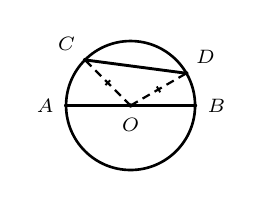
\begin{tikzpicture}[scale=0.39, every node/.style={font=\scriptsize, text=black}]
      \coordinate (O) at (0,0); \def\R{2.1}
      \coordinate (A) at (-\R,0); \coordinate (B) at (\R,0);
      \coordinate (C) at (135:\R); \coordinate (D) at (30:\R);
      \draw[black, line width=0.95pt] (O) circle (\R);
      \draw[black, line width=1.05pt] (A)--(B) (C)--(D);
      \draw[black, line width=0.8pt, densely dashed] (O)--(C) (O)--(D);
      \tickone{O}{C}\tickone{O}{D}
      \fill[black] (O) circle (2pt) (A) circle (1.9pt) (B) circle (1.9pt) (C) circle (1.9pt) (D) circle (1.9pt);
      \node[below=1pt] at (O) {$O$};
      \node[left=1pt] at (A) {$A$}; \node[right=1pt] at (B) {$B$};
      \node[above left=0pt] at (C) {$C$}; \node[above right=0pt] at (D) {$D$};
    \end{tikzpicture}
  \end{minipage}
\end{tcolorbox}

\begin{tcolorbox}[
  enhanced, sharp corners, colback=white, colframe=black,
  boxrule=0.95pt, boxsep=2pt, top=3.5pt, bottom=3.5pt, left=6pt, right=6pt, after skip=4pt
]
  \renewcommand{\arraystretch}{1.18}
  \begin{tabular}{|p{8.7cm}|p{8.7cm}|}
    \hline
    \cellcolor{headgray}\centering\textbf{២. លំហាត់គំរូទី ២ (ទំ.២០១ — $MN = PQ \Rightarrow \arc{MN} = \arc{PQ}$)} &
    \cellcolor{headgray}\centering\arraybackslash\textbf{៣. លំហាត់គំរូទី ៣ (ទំ.២០១ — $\arc{AB} > \arc{CD} \Rightarrow AB > CD$)} \\[2pt]
    \hline
    \begin{minipage}[t]{8.5cm}
      \vspace{2pt}
      \begin{minipage}[c]{3.1cm}
        \centering
        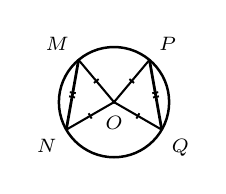
\begin{tikzpicture}[scale=0.35, every node/.style={font=\scriptsize, text=black}]
          \coordinate (O) at (0,0); \def\R{2.0}
          \coordinate (M) at (130:\R); \coordinate (N) at (210:\R);
          \coordinate (P) at (50:\R); \coordinate (Q) at (-30:\R);
          \draw[black, line width=0.9pt] (O) circle (\R);
          \draw[black, line width=1.0pt] (M)--(N) (P)--(Q);
          \draw[black, line width=0.75pt] (O)--(M) (O)--(N) (O)--(P) (O)--(Q);
          \tickone{O}{M}\tickone{O}{N}\tickone{O}{P}\tickone{O}{Q}
          \ticktwo{M}{N}\ticktwo{P}{Q}
          \fill[black] (O) circle (2pt);
          \node[below=1.5pt] at (O) {$O$};
          \node[above left=0pt] at (M) {$M$}; \node[below left=0pt] at (N) {$N$};
          \node[above right=0pt] at (P) {$P$}; \node[below right=0pt] at (Q) {$Q$};
        \end{tikzpicture}
      \end{minipage}\hfill
      \begin{minipage}[c]{5.2cm}
        ក្នុង $\tri{NOM}$ និង $\tri{POQ}$ មាន៖\\
        $\bullet$ $ON = OP = r$ និង $OM =$ \blank{1.0cm} (\cnum{1})\\
        $\bullet$ $MN = PQ$ (សម្មតិកម្ម)\\
        $\Rightarrow \tri{NOM} \cong \tri{POQ}$ (តាម \blank{0.7cm})\\
        $\Rightarrow \angle NOM =$ \blank{1.3cm}\\
        $\Rightarrow \arc{MN} =$ \blank{1.2cm} (តាម \blank{0.7cm})។
      \end{minipage}
      \vspace{2pt}
    \end{minipage}
    &
    \arraybackslash
    \begin{minipage}[t]{8.5cm}
      \vspace{2pt}
      \begin{minipage}[c]{3.1cm}
        \centering
        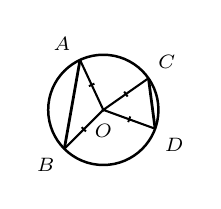
\begin{tikzpicture}[scale=0.35, every node/.style={font=\scriptsize, text=black}]
          \coordinate (O) at (0,0); \def\R{2.0}
          \coordinate (A) at (115:\R); \coordinate (B) at (225:\R);
          \coordinate (C) at (35:\R); \coordinate (D) at (-20:\R);
          \draw[black, line width=0.9pt] (O) circle (\R);
          \draw[black, line width=1.0pt] (A)--(B) (C)--(D);
          \draw[black, line width=0.75pt] (O)--(A) (O)--(B) (O)--(C) (O)--(D);
          \tickone{O}{A}\tickone{O}{B}\tickone{O}{C}\tickone{O}{D}
          \fill[black] (O) circle (2pt);
          \node[below=1.5pt] at (O) {$O$};
          \node[above left=0pt] at (A) {$A$}; \node[below left=0pt] at (B) {$B$};
          \node[above right=0pt] at (C) {$C$}; \node[below right=0pt] at (D) {$D$};
        \end{tikzpicture}
      \end{minipage}\hfill
      \begin{minipage}[c]{5.2cm}
        គេឱ្យធ្នូតូច $\arc{AB} > \arc{CD}$៖\\
        $\bullet$ មុំផ្ចិត $\angle AOB$ \blank{0.7cm} $\angle COD$\\
        $\bullet$ ក្នុង $\tri{AOB}$ និង $\tri{COD}$ មាន៖\\
        $OA = OC = r,\; OB = OD = r$ (\cnum{1})\\
        តាមហេតុផលលេខ \blank{0.8cm} (ត្រចៀកទ្វារ)\\
        គេទាញបានអង្កត់ធ្នូ $AB$ \blank{0.8cm} $CD$។
      \end{minipage}
      \vspace{2pt}
    \end{minipage} \\[3pt]
    \hline
  \end{tabular}
\end{tcolorbox}

% ==================== ផ្នែកទី ៥ ៖ E5 - EVALUATE ====================
\secbar{ផ្នែកទី ៥ ៖ សម្រាយបញ្ជាក់លំហាត់ទី៣ និងបិទបេសកកម្ម (\enbf{E5 — Evaluate})}{\en{10} នាទី (ទំ.២០៤)}

\begin{tcolorbox}[
  enhanced, sharp corners, colback=white, colframe=black,
  boxrule=0.95pt, boxsep=2pt, top=3.5pt, bottom=3.5pt, left=6pt, right=6pt, after skip=4pt
]
  \begin{minipage}[c]{12.6cm}
    \textbf{១. លំហាត់ទី ៣ (ទំ.២០៤ — វិធីបូកធ្នូរួម)៖} ក្នុងរង្វង់ $C(O,r)$ គេមានអង្កត់ធ្នូ $AB = CD$ ដូចរូបខាងស្ដាំ។ ចូរបង្ហាញថាធ្នូ $\arc{AC} = \arc{BD}$៖
    \begin{itemize}[leftmargin=1.2em, itemsep=2.5pt, topsep=1.5pt]
      \item ដោយអង្កត់ធ្នូ $AB = CD$ (សម្មតិកម្ម) តាមទ្រឹស្ដីបទ ២ គេបានធ្នូ $\arc{AB} =$ \blank{1.4cm}។
      \item បូកធ្នូរួម $\arc{BC}$ ទៅនឹងអង្គទាំងពីរនៃសមភាព៖ $\arc{AB} + \blank{1.2cm} = \arc{CD} + \blank{1.2cm}$។
      \item ដោយ $\arc{AB} + \arc{BC} = \arc{AC}$ និង $\arc{CD} + \arc{BC} =$ \blank{1.4cm} ដូចនេះគេបាន \textbf{$\arc{AC} = \arc{BD}$} (ហើយអង្កត់ធ្នូ $AC =$ \blank{1.2cm})។
    \end{itemize}
  \end{minipage}\hfill
  \begin{minipage}[c]{5.2cm}
    \centering
    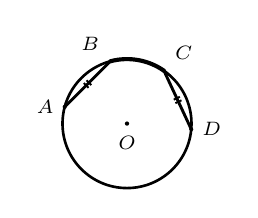
\begin{tikzpicture}[scale=0.39, every node/.style={font=\scriptsize, text=black}]
      \coordinate (O) at (0,0); \def\R{2.1}
      \coordinate (A) at (165:\R); \coordinate (B) at (105:\R);
      \coordinate (C) at (55:\R); \coordinate (D) at (-5:\R);
      \draw[black, line width=0.95pt] (O) circle (\R);
      \draw[black, line width=1.05pt] (A)--(B) (C)--(D);
      \draw[black, line width=1.5pt] (C) arc (55:105:\R);
      \ticktwo{A}{B}\ticktwo{C}{D}
      \fill[black] (O) circle (2pt) (A) circle (1.9pt) (B) circle (1.9pt) (C) circle (1.9pt) (D) circle (1.9pt);
      \node[below=1pt] at (O) {$O$};
      \node[left=0.5pt] at (A) {$A$}; \node[above left=0.5pt] at (B) {$B$};
      \node[above right=0.5pt] at (C) {$C$}; \node[right=0.5pt] at (D) {$D$};
    \end{tikzpicture}
  \end{minipage}
\end{tcolorbox}

\begin{tcolorbox}[
  enhanced, sharp corners, colback=white, colframe=black,
  boxrule=0.95pt, boxsep=2pt, top=3.5pt, bottom=3.5pt, left=6pt, right=6pt, after skip=4pt
]
  \textbf{២. បិទបេសកកម្ម E1 (ចង្អេរឫស្សី $r = 25\unit{cm}$)៖} ត្រូវដាក់របារឫស្សីកាត់តាមផ្ចិត $O$ ជា \textbf{អង្កត់ផ្ចិត} ដែលមានប្រវែងវែងបំផុតស្មើនឹង $d = 2r =$ \blank{1.5cm} $\unit{cm}$ ហើយបើធ្នូ $\arc{CF} = 2\arc{CD}$ នោះអង្កត់ធ្នូ $CF$ \blank{0.8cm} $2CD$!\\[2.5pt]
  \textbf{៣. Exit Check (៦០ វិនាទី)៖} ក្នុងរង្វង់ $C(O, 6\unit{cm})$ តើអង្កត់ធ្នូធំបំផុតមានប្រវែងប៉ុន្មាន ហើយបើធ្នូតូច $\arc{PQ} = 2\arc{RS}$ តើប្រវែងអង្កត់ធ្នូប្រៀបធៀបយ៉ាងដូចម្ដេច?\\
  \chkbox\ \textbf{A.} $12\unit{cm}$ និង $PQ < 2RS$ \hspace{0.35cm}
  \chkbox\ \textbf{B.} $12\unit{cm}$ និង $PQ = 2RS$ \hspace{0.35cm}
  \chkbox\ \textbf{C.} $6\unit{cm}$ និង $PQ < 2RS$ \hspace{0.35cm}
  \chkbox\ \textbf{D.} $12\unit{cm}$ និង $PQ > 2RS$
\end{tcolorbox}

% ==================== កិច្ចការផ្ទះ (ជំហានទី ៥) ====================
\begin{tcolorbox}[
  enhanced, sharp corners, colback=panelgray, colframe=black,
  boxrule=1.0pt, boxsep=2pt, top=3.5pt, bottom=3.5pt, left=6pt, right=6pt
]
  {\muol\fontsize{9.0pt}{13pt}\selectfont កិច្ចការផ្ទះ (សៀវភៅសិក្សាគោល ទំព័រ ២០៤ — ត្រៀមអានចំណុច ២.២ ទំព័រ ២០២--២០៣)}\\[2pt]
  $\bullet$ \textbf{លំហាត់ទី ២ (ទំ.២០៤)៖} ក្នុងរង្វង់ $C(O,r)$ គេមានធ្នូ $\arc{AD} = \arc{CB}$។ ចូរបង្ហាញថាអង្កត់ធ្នូ $AD = CB$ (ព្រមទាំងស្រាយបញ្ជាក់បន្ថែមក្នុងករណីគេឱ្យធ្នូ $\arc{AC} = \arc{BD}$ ដោយបូកធ្នូរួម $\arc{CD}$ ទាំងសងខាង)។\\
  $\bullet$ \textbf{លំហាត់ទី ៥ (ទំ.២០៤)៖} ក្នុងរង្វង់ $C(O,r)$ គេឱ្យអង្កត់ធ្នូ $AB = CD$។ ចូរបង្ហាញថាធ្នូ $\arc{BD} = \arc{AC}$ (ណែនាំ៖ ប្រើទ្រឹស្ដីបទ ២ រួចបូក ឬដកធ្នូរួម)។
\end{tcolorbox}

\end{document}
